\chapter{Abstract models for true concurrency}
\label{chap:absmod}



In this chapter, we look at classical models of true concurrency. Starting in Section \ref{sub:tradisys} with classical transition systems and their interleaving semantics, we look at different ways to add true concurrency in the picture, especially by specifying that transitions, actions or events are independent (asynchronous systems \ref{subsec:ats}, transition systems with independence \ref{subsec:tsi}). In Section \ref{sec:bists}, we look at bisimulations for transition systems: they are a classical way to say that two systems have the same computational behavior. We make an overview of the different equivalent formulations of this equivalence relation (game theoretic, logical, ...). After that, in Section \ref{sec:semtc} we look at extensions of bisimulations for true concurrency, in the case of transition systems with independence, by unfolding such systems to event structures. We also look at action refinements, an important feature of true concurrency in Section \ref{subsec:actref}: if two systems are equivalent, they are equivalent whatever is the granularity of actions. In Section \ref{sec:hda}, we start our tour to geometry: higher dimensional automata are a powerful model for true concurrency which is geometric. Concurrent behaviors are modeled by higher-dimensional cells that can be interpreted geometrically as we will see in the next chapter. Finally, in Section \ref{sec:supv}, we describe two concrete languages, PV and SU-programs, and their translation in abstract models.




\section{Transition systems and variants}

In this section, we start by recalling a few transition systems for modeling concurrency, along with their executions and simulations.

	\subsection{Traditional systems}
	\label{sub:tradisys}
	
	Transition systems are the simplest models of computations. They consist of a transition graph, that is, objects which represent the states of the system and transitions which model the change of state of the system due to particular events.
	
	Fix a set $\Sigma$, called the \textbf{alphabet}. A ($\Sigma$-)\textbf{transition system} is a tuple $T = (Q,i,\Delta)$ where:
	\begin{itemize}
		\item $Q$ is a set (of \textbf{states}),
		\item $i$ is a element of $Q$ (called the \textbf{initial state}),
		\item $\Delta$ is a subset of $Q\times\Sigma\times Q$ (\textbf{transitions}).
	\end{itemize}
	
	
\noindent A \textbf{morphism $f$ of transition systems} from $T = (Q,i,\Delta)$ to $S = (Q',i',\Delta')$ is a function $$\map{f}{Q}{Q'}$$ such that:
	\begin{itemize}
		\item $f(i) = i'$,
		\item for every transition $(q,a,q') \in \Delta$, $(f(q),a,f(q')) \in \Delta'$.
	\end{itemize}
	$\Sigma$-transition systems, together with morphisms of transition systems form a category, noted $\tr$.

	
	 Morphisms act like particular simulations, in the sense that if $\map{f}{T}{S}$ is a morphism of transition systems, then $S$ contains (at least) the computational behavior of $T$. First, executions of $T$ can be simulated in $S$. To be more precise, an \textbf{execution} of $T = (Q,i,\Delta)$ is a finite sequence:
	 $$q_0 \xrightarrow{~a_1~} q_1 \xrightarrow{~a_2~} \ldots \xrightarrow{~a_n~} q_n$$
	 where $q_0 = i$ is the initial state of $T$ and for every $j \in \{1, \ldots, n\}$, $(q_{j-1},a_j,q_j) \in \Delta$. Executions can be seen as particular morphisms. A \textbf{branch} is a transition system of the form $B = (\textbf{[n]},0,\Lambda)$ where:
	 \begin{itemize}
	 	\item $\textbf{[n]} = \{0,1,\ldots,n\}$,
		\item for every $j \in \{1, \ldots, n\}$, there is a unique transition of the form $(j-1,a_j,j)$ in $\Lambda$, for some $a_1, \ldots, a_n \in \Sigma$.
	\end{itemize}
	Then an execution of $T$ is exactly a morphism from a branch to $T$. So if $\map{p}{B}{T}$ is an execution of $T$ and $\map{f}{T}{S}$ is a morphism of transition systems, then $f\circ p$ is an execution of $S$. Actually, this statement can be made even more precise, by using the notion of \textbf{simulation}. A simulation from $T = (Q,i,\Delta)$ to $S = (Q',i',\Delta')$ is a relation $R \subseteq Q\times Q'$ such that:
	\begin{itemize}
		\item $(i,i') \in R$,
		\item for every $(q,q') \in R$, and every transition $(q,a,p)$ in $T$, there is a transition $(q',a,p')$ in $S$ such that $(p,p') \in R$.
	\end{itemize}
	When such a simulation exists, we say that \textbf{$T$ is simulated by $S$}.
	
	A morphism $\map{f}{T}{S}$ induces a simulation $R = \{(q,f(q)) \mid q \in Q\}$. When $T$ is simulated by $S$ then the executions of $T$ are contained in the executions of $S$, but the converse is false. Consider for example, the following two transition systems:
	
	
	\begin{figure}[H]
		\begin{center}
    			
\begin{tikzpicture}[scale=1]
		
	\node (1) at (0,0) {$q_1$};
	\node (2) at (-1,-1.5) {$q_2$};
	\node (4) at (1,-1.5) {$q_4$};
	\node (3) at (-1,-3) {$q_3$};
	\node (5) at (1, -3) {$q_5$};
	
	\node (1p) at (6,0) {$q'_1$};
	\node (2p) at (6,-1.5) {$q'_2$};
	\node (3p) at (5,-3) {$q'_3$};
	\node (5p) at (7,-3) {$q'_5$};
	
	\path[->,font=\scriptsize]
		(0,0.5) edge (1)
		(1) edge node[left]{$a$} (2)
		(1) edge node[right]{$a$} (4)
		(2) edge node[left]{$b$} (3)
		(4) edge node[right]{$c$} (5)
		
		(6,0.6) edge (1p)
		(1p) edge node[left]{$a$} (2p)
		(2p) edge node[left]{$b$} (3p)
		(2p) edge node[right]{$c$} (5p);
		
	\path[->, dotted, bend left = 20]
		(1) edge (1p)
		(2) edge (2p)
		(4) edge (2p)
		(3) edge (3p)
		(5) edge (5p);
			
\end{tikzpicture}


  		\end{center}
  		\caption{Two transition systems $T$ (on the left) and $S$ (on the right),\\and a morphism from $T$ to $S$}
	\end{figure}


	There is a morphism from $T$ to $S$ which maps $q_2$ and $q_4$ to $q'_2$, they have the same executions, namely $0 \xrightarrow{~a~} 1 \xrightarrow{~b~} 2$ and $0 \xrightarrow{~a~} 1 \xrightarrow{~c~} 2$, but there is no simulation from $S$ to $T$. Indeed, if there were some, say $R$, we must have $(q'_1,q_1) \in R$. Then since $(q'_1,a,q'_2)$ is a transition of $S$ there must be $q$ state of $T$ and a transition $(q_1,a,q)$ in $T$ with $(q'_2,q) \in R$. So $q$ can only be $q_2$ or $q_4$. If it is $q_2$, since $(q'_2,c,q'_5)$ is a transition of $S$, there must be a transition $(q_2,c,q')$ in $T$ for some $q'$, which is not the case. Similarly if it is $q_4$.
	
	Transition systems can model interleaving behaviors of concurrency. Let us illustrate this on an example. Assume that we have two processes $A$ and $B$ executing in parallel. $A$ wants to change the value of a variable $X$ to $0$ and $B$ wants to change the value of $Y$ to $1$. The behavior of those processes can be modeled by the following transition system:
	
	
	\begin{figure}[!htbp]
		\begin{center}
    			
\begin{tikzpicture}[scale=1]
		
	\node (1) at (0,0) {$q_\varnothing$};
	\node (2) at (3,0) {$q_A$};
	\node (4) at (0,3) {$q_B$};
	\node (3) at (3,3) {$q_{A,B}$};
	
	\path[->,font=\scriptsize]
		(-0.5,-0.5) edge (1)
		(1) edge node[below]{$X := 0$} (2)
		(1) edge node[left]{$Y := 1$} (4)
		(2) edge node[right]{$Y := 1$} (3)
		(4) edge node[above]{$X := 0$} (3);
			
\end{tikzpicture}


  		\end{center}
  		\caption{A transition system modeling two processes executing an action in parallel}
  		\label{fig:jolieImage}
	\end{figure}
	
	Intuitively, $q_\varnothing$ corresponds to the state where neither $A$ nor $B$ have done their action, $q_A$ (resp. $q_B$) to the state where $A$ (resp. $B$) has done its action but not $B$ (resp. $A$), and $q_{A,B}$ to the state where both $A$ and $B$ have done their action. So the different behaviors modeled by this transition system are that $A$ can do its action before $B$ or vice versa, that is, executions of this system are interleaving of executions of $A$ and $B$. There is no way to model that $A$ and $B$ execute \emph{simultaneously}.
	
	
	\subsection{Asynchronous transition systems}
	\label{subsec:ats}
	
	To solve this problem, one extends the notion of executions to take into account that two actions can be made simultaneously. But one must be careful because not just any actions can be executed simultaneously. Indeed, in the first example, if $X$ and $Y$ are the same variable, executing $X := 0$ and $Y := 1$ may lead to unexpected results. So one must declare beforehand which are the actions that can be done simultaneously. 
	

	A ($\Sigma$-)\textbf{asynchronous transition system} \cite{shields85,bednarczyk87} $(Q,i,\Delta,\lambda,I)$ is the following data:
		\begin{itemize}
			\item a function $\map{\lambda}{E}{\Sigma}$. $E$ is called the set of \textbf{events} and $\lambda$ associates an event with the action it induces.
			\item a $E$-transition system $(Q,i,\Delta\subseteq Q\times E \times Q)$,
			\item an irreflexive and symmetric relation $I \subseteq E^2$ (\textbf{independence relation}),
		\end{itemize}
		
\noindent such that:
		
		\begin{itemize}
			\item[i)] for every $e \in E$, there are states $q$, $q' \in Q$ with $(q,e,q') \in \Delta$,
			\item[ii)] for every pair $(q,e,q')$ and $(q,e,q'')$ of transitions, $q' = q''$, 
			\item[iii)] for every pair $(q,e,q')$ and $(q,e',q'')$ of transitions with $(e,e') \in I$, there is a pair of transitions $(q',e',p)$ and $(q'',e,p)$ for some state $p$,
			
				\begin{figure}[H]
					\begin{center}
    						
\begin{tikzpicture}[scale=1]
		
	\node (q) at (0,0) {$q$};
	\node (q') at (0,3) {$q'$};
	\node (q'') at (3,0) {$q''$};
	\node (p) at (3,3) {$p$};
	
	
	\path[->,font=\scriptsize]
		(q) edge node[left]{$e$} (q')
		(q) edge node[below]{$e'$} (q'');
		
	\path[->, dotted, font=\scriptsize]
		(q'') edge node[right]{$e$} (p)
		(q') edge node[above]{$e'$} (p);
			
\end{tikzpicture}


  					\end{center}
				\end{figure}
			
			\item[iv)] for every pair $(q,e,q')$ and $(q',e',q'')$ of transitions with $(e,e') \in I$, there is a pair of transitions $(q,e',p)$ and $(p,e,q'')$ for some state $p$.
			
				\begin{figure}[H]
					\begin{center}
    						
\begin{tikzpicture}[scale=1]
		
	\node (q) at (0,0) {$q$};
	\node (q') at (0,3) {$q'$};
	\node (p) at (3,0) {$p$};
	\node (q'') at (3,3) {$q''$};
	
	
	\path[->,font=\scriptsize]
		(q) edge node[left]{$e$} (q')
		(q') edge node[above]{$e'$} (q'');
		
	\path[->, dotted, font=\scriptsize]
		(q) edge node[below]{$e'$} (p)
		(p) edge node[right]{$e$} (q'');
			
\end{tikzpicture}


  					\end{center}
				\end{figure}
		\end{itemize}

	
	An asynchronous transition system is then a transition system which is deterministic with respect to events and for which one can declare that two events can occur simultaneously. Indeed, if two events are independent, the axioms $iii)$ and $iv)$ provide that those events can occur in any order, in particular simultaneously. 
	

	A \textbf{morphism $(f,g)$ of asynchronous transition systems} from $(Q,i,\Delta,\map{\lambda}{E}{\Sigma},I)$ to $(Q',i',\Delta',\map{\lambda'}{E'}{\Sigma},I')$ is a pair of functions $\map{f}{Q}{Q'}$ and $\map{g}{E}{E'}$ such that:
		\begin{itemize}
			\item $\lambda'\circ g = \lambda$,
			\item $f(i) = i'$,
			\item for every transition $(q,e,q') \in \Delta$, $(f(q),g(e),f(q')) \in \Delta'$.
		\end{itemize}
	We note $\astr$ the category of asynchronous transition systems and morphisms of transition systems.

	
	
	We can now update the example of the introduction of this section. In this case, events are actions. We need to declare an independence relation on the set of events $\{X:=0,Y:=1\}$. If $X$ and $Y$ are distinct variables, we can execute both events simultaneously and we can define $I = \{(X:=0,Y:=1),(Y:=1, X:=0)\}$.
	
	The interest of events over actions is that we can model the following behavior:
	
		\begin{figure}[H]
			\begin{center}
    				
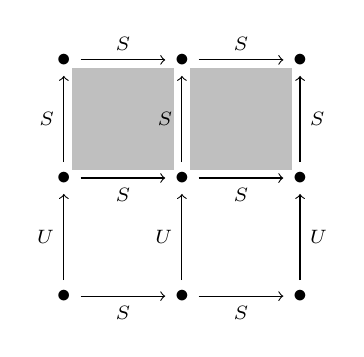
\begin{tikzpicture}[scale=1]
		
	\node (11) at (0,0) {$\bullet$};
	\node (12) at (0,1.5) {$\bullet$};
	\node (13) at (0,3) {$\bullet$};
	\node (21) at (1.5,0) {$\bullet$};
	\node (22) at (1.5, 1.5) {$\bullet$};
	\node (23) at (1.5,3) {$\bullet$};
	\node (31) at (3,0) {$\bullet$};
	\node (32) at (3,1.5) {$\bullet$};
	\node (33) at (3,3) {$\bullet$};
	
	\draw[draw = white, fill = gray!50] (0.1,1.6) rectangle (1.4,2.9);
	\draw[draw = white, fill = gray!50] (1.6,1.6) rectangle (2.9,2.9);
	
	\path[->,font=\scriptsize]
		(11) edge node[left]{$U$} (12)
		(12) edge node[left]{$S$} (13)
		(21) edge node[left]{$U$} (22)
		(22) edge node[left]{$S$} (23)
		(31) edge node[right]{$U$} (32)
		(32) edge node[right]{$S$} (33)
		(11) edge node[below]{$S$} (21)
		(21) edge node[below]{$S$} (31)
		(12) edge node[below]{$S$} (22)
		(22) edge node[below]{$S$} (32)
		(13) edge node[above]{$S$} (23)
		(23) edge node[above]{$S$} (33);
			
\end{tikzpicture}


  			\end{center}
		\end{figure}
	
	You may think it as two processes executing actions in parallel, which are of two kinds $S$ and $U$ (see later for their actual meaning), such that $U$ and $S$ cannot be executed simultaneously, but $U$ and $U$ (resp. $S$ and $S$) can. So we will be able to model it with this asynchronous transition system:
	
		\begin{figure}[H]
			\begin{center}
    				
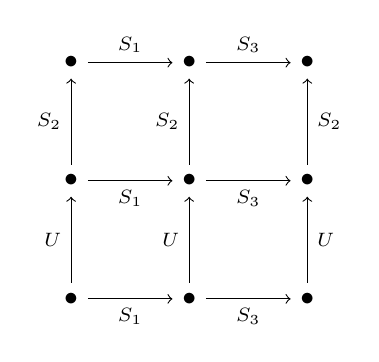
\begin{tikzpicture}[scale=1]
		
	\node (11) at (0,0) {$\bullet$};
	\node (12) at (0,1.5) {$\bullet$};
	\node (13) at (0,3) {$\bullet$};
	\node (21) at (1.5,0) {$\bullet$};
	\node (22) at (1.5, 1.5) {$\bullet$};
	\node (23) at (1.5,3) {$\bullet$};
	\node (31) at (3,0) {$\bullet$};
	\node (32) at (3,1.5) {$\bullet$};
	\node (33) at (3,3) {$\bullet$};
	
	
	\path[->,font=\scriptsize]
		(11) edge node[left]{$U$} (12)
		(12) edge node[left]{$S_2$} (13)
		(21) edge node[left]{$U$} (22)
		(22) edge node[left]{$S_2$} (23)
		(31) edge node[right]{$U$} (32)
		(32) edge node[right]{$S_2$} (33)
		(11) edge node[below]{$S_1$} (21)
		(21) edge node[below]{$S_3$} (31)
		(12) edge node[below]{$S_1$} (22)
		(22) edge node[below]{$S_3$} (32)
		(13) edge node[above]{$S_1$} (23)
		(23) edge node[above]{$S_3$} (33);
			
\end{tikzpicture}


  			\end{center}
		\end{figure}
	
\noindent with $S_1$, $S_2$ and $S_3$ pairwise independent. Intuitively, the event $S_1$ (resp. $S_3$) means that the first process executes its first (resp. second) $S$ action, while $S_2$ means that the second process executes its $S$ action. So for example, every $S_1$-transition models the same event whose induced action is an $S$-action. They only differ on where the second process is in its own execution.
	
	We can now extend the notion of executions to handle simultaneous behaviors. A \textbf{trace} on $\Sigma$ is a word on $\text{Mul}(\Sigma)$ the set of finite multisets of $\Sigma$. A \textbf{trace language} $M$ is a set of traces on $\Sigma$ such that:
		\begin{itemize}
			\item if $u.S \in M$, with $S \in \text{Mul}(\Sigma)$ and $u$ a trace, then $u \in M$ (closure under prefix).
			\item if $u.(S_1 + S_2).v \in M$, with $S_1, S_2 \in \text{Mul}(\Sigma)$ and $u$, $v$ traces, then $u.S_1.S_2.v \in M$.
		\end{itemize}

	
An asynchronous transition system induces a trace language as follow. Define a \textbf{cube} as an asynchronous transition system of the form:
\begin{itemize}
	\item its states are $\{0,1\}^n$ for some $n$, 
	\item its initial state is $(0, \ldots, 0)$,
	\item its set of events is $\{1, ..., n\}$,
	\item its transitions are of the form $(v,i,v+e_i)$ where $e_i$ is the vector with $0$ everywhere except the $i$th coordinate which is $1$,
	\item $I$ is $\{(i,j) \mid i \neq j\}$,
	\item $\lambda$ is anything you want.
\end{itemize}

		\begin{figure}[H]
			\begin{center}
    				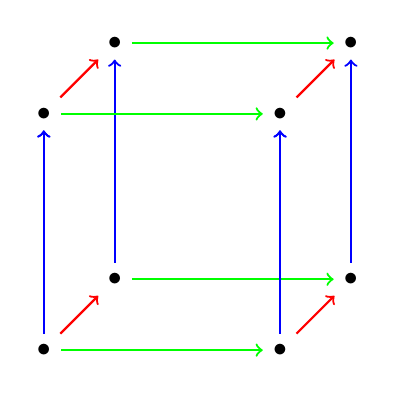
\begin{tikzpicture}[thick,scale=3]

    	\node (A1) at (0, 0) {$\bullet$};
    	\node (A2) at (0, 1) {$\bullet$};;
    	\node (A3) at (1, 1) {$\bullet$};;
    	\node (A4) at (1, 0) {$\bullet$};;
    	\node (B1) at (0.3, 0.3) {$\bullet$};;
    	\node (B2) at (0.3, 1.3) {$\bullet$};;
    	\node (B3) at (1.3, 1.3) {$\bullet$};;
    	\node (B4) at (1.3, 0.3) {$\bullet$};;
		
	\path[->,font=\scriptsize, draw = blue]
		(B1) edge (B2)
		(B4) edge (B3);
		
	\path[->,font=\scriptsize, draw = green]
		(B1) edge (B4)
		(B2) edge (B3);
		
	\path[->,font=\scriptsize, draw = blue]
		(A1) edge (A2)
		(A4) edge (A3);
		
	\path[->,font=\scriptsize, draw = green]
		(A1) edge (A4)
		(A2) edge (A3);
		
	\path[->,font=\scriptsize, draw = blue]
		(A1) edge (A2)
		(A4) edge (A3);
		
	\path[->,font=\scriptsize, draw = red]
		(A1) edge (B1)
		(A2) edge (B2)
		(A3) edge (B3)
		(A4) edge (B4);
		
\end{tikzpicture}
  			\end{center}
  			\caption{A cube for $n = 3$ ; each color corresponds to an event.}
		\end{figure}

An \textbf{asynchronous branch} is then the concatenation of cubes (identifying the upper corner of one cube with the lower corner of the following). For example, this is an asynchronous branch:

		\begin{figure}[H]
			\begin{center}
    				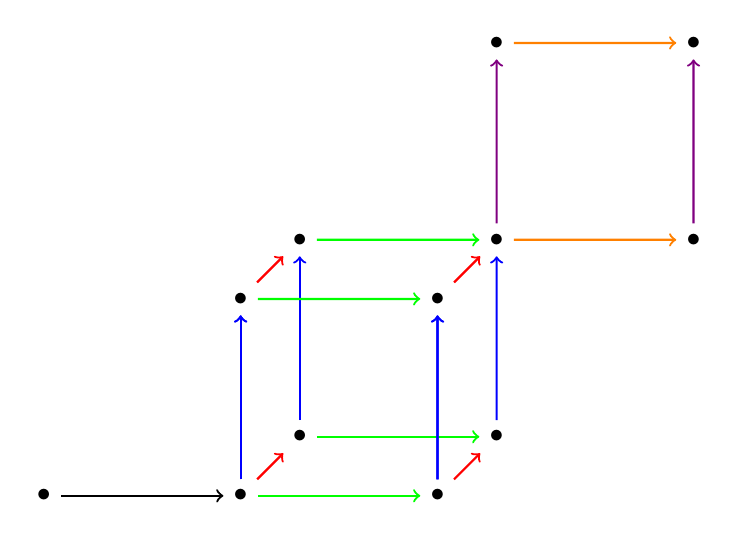
\begin{tikzpicture}[thick,scale=2.5]

    	\node (C0) at (-1,0) {$\bullet$};
	\node (A1) at (0, 0) {$\bullet$};
    	\node (A2) at (0, 1) {$\bullet$};
    	\node (A3) at (1, 1) {$\bullet$};
    	\node (A4) at (1, 0) {$\bullet$};
    	\node (B1) at (0.3, 0.3) {$\bullet$};
    	\node (B2) at (0.3, 1.3) {$\bullet$};
    	\node (B3) at (1.3, 1.3) {$\bullet$};
    	\node (B4) at (1.3, 0.3) {$\bullet$};
	\node (D2) at (1.3, 2.3) {$\bullet$};
	\node (D3) at (2.3, 2.3) {$\bullet$};
	\node (D4) at (2.3, 1.3) {$\bullet$};
	
	\path[->]
		(C0) edge (A1);
		
	\path[->, draw = blue]
		(B1) edge (B2)
		(B4) edge (B3);
		
	\path[->, draw = green]
		(B1) edge (B4)
		(B2) edge (B3);
		
	\path[->, draw = blue]
		(A1) edge (A2)
		(A4) edge (A3);
		
	\path[->, draw = green]
		(A1) edge (A4)
		(A2) edge (A3);
		
	\path[->, draw = blue]
		(A1) edge (A2)
		(A4) edge (A3);
		
	\path[->, draw = red]
		(A1) edge (B1)
		(A2) edge (B2)
		(A3) edge (B3)
		(A4) edge (B4);
		
	\path[->, draw = violet]
		(B3) edge (D2)
		(D4) edge (D3);
		
	\path[->, draw = orange]
		(B3) edge (D4)
		(D2) edge (D3);

\end{tikzpicture}





  			\end{center}
  			\caption{An asynchronous branch.}
		\end{figure}

The trace induced by an asynchronous branch $c_1, ..., c_n$ is defined as $S_1. \ldots . S_n$ where $S_i$ is the image of the $\lambda$ function in the cube $c_i$. An asynchronous execution of an asynchronous transition system $T$ is a morphism from an asynchronous branch to $T$. The trace language induced by $T$ is then the set of traces induced by its asynchronous executions (it is easy to check that it is actually a trace language). When there is a morphism from $T$ to $S$ then the trace language of $T$ is included in $S$.

The idea is similar to Mazurkiewicz traces \cite{mazurkiewicz89}, although the definition is a bit different.
	
	
	
	
	\subsection{Transition system with independence}
	\label{subsec:tsi}
	
	In asynchronous transition systems, we specify simultaneity by refining the notion of actions by, intuitively, regrouping transitions which represent the same event, possibly in a different context. Those events were explicit and independence was defined on those events. In this subsection, we present an extension of transition systems from \cite{nielsen94} in which one can define independence directly on transitions and where events are implicit and can be defined afterwards.
	
	A \textbf{transition system with independence} $(Q, i, \Delta, I)$ is:
		\begin{itemize}
			\item a $\Sigma$-transition system $(Q, i, \Delta)$,
			\item an irreflexive symmetric relation $I \subseteq \Delta^2$ (\textbf{independence relation}).
		\end{itemize}
	Define $\prec \,\subseteq \,\Delta\times\Delta$ as:
	$$(q,a,q') \prec (p,a,p') \text{ iff } \exists b.\, ((q,a,q'),(q,b,p)), ((q,a,q'),(q',b,p')), ((q,b,p),(p,a,p')) \in I$$
	
				\begin{figure}[H]
					\begin{center}
    						
\begin{tikzpicture}[scale=1]
		
	\node (q) at (0,0) {$q$};
	\node (q') at (3,0) {$q'$};
	\node (p) at (0,3) {$p$};
	\node (p') at (3,3) {$p'$};
	
	\path[dotted, bend right = 45]
		(0.5,0.1) edge (0.1,0.5)
		(0.1,2.5) edge (0.5,2.9)
		(2.9,0.5) edge (2.5,0.1);
	
	\path[->,font=\scriptsize]
		(q) edge node[below]{$a$} (q')
		(p) edge node[above]{$a$} (p');
		
	\path[->, dotted, font=\scriptsize]
		(q) edge node[left]{$b$} (p)
		(q') edge node[right]{$b$} (p');
			
\end{tikzpicture}


  					\end{center}
				\end{figure}
	
\noindent and let $\sim$ be the least equivalence relation which contains $\prec$. We call \textbf{events} the equivalence classes of $\sim$. Those data must satisfy the following properties:
		\begin{itemize}
			\item[i)] if $(q,a,q') \sim (q,a,q'')$, then $q' = q''$,
			\item[ii)] if $((q,a,q'),(q',b,q''))\in I$, then there exists a state $p$ such that $((q,a,q'),(q,b,p)) \in I$ and $((q,b,p),(p,a,q'')) \in I$,
			
				\begin{figure}[H]
					\begin{center}
    						
\begin{tikzpicture}[scale=1]
		
	\node (q) at (0,0) {$q$};
	\node (q') at (3,0) {$q'$};
	\node (q'') at (0,3) {$q''$};
	\node (p) at (3,3) {$p$};
	
	\path[dotted, bend right = 45]
		(0.1,2.5) edge (0.5,2.9)
		(2.9,0.5) edge (2.5,0.1);
		
	\path[bend left = 45]
		(0.1,0.5) edge (0.5,0.1);
	
	\path[->,font=\scriptsize]
		(q) edge node[below]{$a$} (q')
		(q) edge node[left]{$b$} (q'');
		
	\path[->, dotted, font=\scriptsize]
		(q') edge node[right]{$b$} (p)
		(q'') edge node[above]{$a$} (p);
			
\end{tikzpicture}


  					\end{center}
				\end{figure}
			
			\item[iii)] if $(q,a,q') \prec (p,a,p')$ and $((p,a,p'),(s,b,s')) \in I$, then $((q,a,q'),(s,b,s')) \in I$,
			\item[iv)] if $(q,a,q') \prec (p,a,p')$ and $((q,a,q'),(s,b,s')) \in I$, then $((p,a,p'),(s,b,s')) \in I$.
		\end{itemize}

	The small arcs in the two previous pictures denote that the transitions linked by it are independent. Axiom $i)$ means that those systems are deterministic with respect to events. Axiom $ii)$ is the property we expect of independence, that is, if two transitions are independent, they can be done in any order we want. Axioms $iii)$ and $iv)$ mean that independence can be defined on events, that is, is compatible with $\sim$. With those events and this extended independence relation, one defines an asynchronous transition system. The diamonds given by axiom $ii)$ give rise to a relation on executions, namely, the smallest equivalence relation $\simeq$ on executions which relates execution of the form:
	 $$q_0 \xrightarrow{~a_1~} q_1 \xrightarrow{~~~~} \ldots q_i \xrightarrow{~a_{i+1}~} q_{i+1}  \xrightarrow{~a_{i+2}~} q_{i+2} \xrightarrow{~~~~} \ldots \xrightarrow{~a_n~} q_n$$
	 $$q_0 \xrightarrow{~a_1~} q_1 \xrightarrow{~~~~} \ldots q_i \xrightarrow{~a_{i+2}~} q'_{i+1}  \xrightarrow{~a_{i+1}~} q_{i+2} \xrightarrow{~~~~} \ldots \xrightarrow{~a_n~} q_n$$
\noindent with the following diamond:
				\begin{figure}[H]
					\begin{center}
    						
\begin{tikzpicture}[scale=1]
		
	\node (q) at (0,0) {$q_i$};
	\node (q') at (3,0) {$q_{i+1}$};
	\node (q'') at (0,3) {$q'_{i+1}$};
	\node (p) at (3,3) {$q_{i+2}$};
	
	\path[bend right = 45]
		(0.1,2.5) edge (0.5,2.9)
		(2.9,0.5) edge (2.5,0.1);
		
	\path[bend left = 45]
		(0.1,0.5) edge (0.5,0.1);
	
	\path[->,font=\scriptsize]
		(q) edge node[below]{$a_{i+1}$} (q')
		(q) edge node[left]{$a_{i+2}$} (q'')
		(q') edge node[right]{$a_{i+2}$} (p)
		(q'') edge node[above]{$a_{i+1}$} (p);
			
\end{tikzpicture}


  					\end{center}
				\end{figure}
%	
%	\subsection{Petri-nets}
%
%	\begin{defi}
%	A \textbf{Petri net} is a tuple $(Q, M_0, T, \lambda, \text{pre}, \text{post})$ where:
%		\begin{itemize}
%			\item $Q$ is a set (of \textbf{places} or \textbf{conditions}),
%			\item $M_0$ is a subset of $P$ (\textbf{initial marking}),
%			\item $T$ is a set (of \textbf{transitions} or \textbf{events},
%			\item $\lambda$ is a function from $T$ to $\Sigma$ (\textbf{labelling}),
%			\item $\textbf{pre}$ is a function from $T$ to $\mathcal{P}(Q)$ (\textbf{precondition}),
%			\item $\textbf{post}$ is a function from $T$ to $\mathcal{P}(Q)$ (\textbf{postcondition}).
%		\end{itemize}
%	\end{defi}
%
%	A \textbf{marking} is a subset of $Q$. We say that there is a transition $e \in T$ from the marking $M$ to the marking $M'$, and we note $M \xrightarrow{~e~} M'$, if $\text{pre}(e) \subseteq M$, $\text{post}(e) \subseteq M'$ and $M'\setminus \text{post}(e) = M\setminus\text{pre}(e)$. We say that a marking is \textbf{accessible} if there is a sequence of transitions from $M_0$ to this marking. What might occur is that $\text{pre}(e) \subseteq M$ and $\text{post}(e) \cap (M \setminus \text{pre}(e)) \neq \varnothing$, and so if we think those transitions as the moving of some tokens on places, we would expect that $M'$ has two tokens on this intersection, which is impossible since markings are sets (and not multisets). In classical Petri nets, when such a phenomenon occurs for an accessible marking, this means that the net is not \textbf{1-safe}. In the following, we will suppose that our nets are \textbf{1-safe}, i.e., for every accessible marking $M$, there is no transition $e$ such that  $\text{pre}(e) \subseteq M$ and $\text{post}(e) \cap (M \setminus \text{pre}(e)) \neq \varnothing$.
%	
%	The notion of morphisms of Petri nets is a bit complex. Since one is expecting that \textit{transitions} are preserved, the naive definition by requiring that a morphism is pair of functions, one between places, one between transitions, with some compatibility conditions does satisfy this property. There were a few different definitions \cite{}. The one will use is the following:
%	
%	\begin{defi}
%	A morphism of Petri nets between $N = (Q, M_0, T, \lambda, \text{pre}, \text{post})$ and $N' = (Q', M'_0, T', \lambda', \text{pre'}, \text{post'})$ is a pair $(\beta,\eta)$ with:
%		\begin{itemize}
%			\item $\beta \subseteq Q\times Q'$, a relation whose opposite relation $\beta^{-1} \subseteq Q'\times Q$ is a partial function, that is, for every $q' \in Q'$, there is at most one $q \in Q$ such that $(q,q') \in \beta$,
%			\item a function $\eta$ from $T$ to $T'$,
%		\end{itemize}
%		satisfying:
%		\begin{itemize}
%			\item $\beta(M_0) = \{q' \in Q' \mid \exists q \in M_0, \, (q,q') \in \beta\} = M'_0$,
%			\item $\beta(\text{pre}(e)) = \text{pre'}(\eta(e))$,
%			\item $\beta(\text{post}(e)) = \text{post'}(\eta(e))$,
%			\item $\lambda'\circ\eta = \lambda$.
%		\end{itemize}
%	We note $\PN$, the category of Petri nets and morphisms.
%	\end{defi}
%	
%	As announced, when $M \xrightarrow{~e~} M'$ in $N$ and if $(\beta,\eta)$ is a morphism from $N$ to $N'$, then $\beta M \xrightarrow{~\eta(e)~} \beta M'$ in $N'$. In particular, if $M$ is accessible in $N$ then $\beta M$ is accessible in $N'$ and the executions of $N$ can be simulated in $N'$.
%	
%	In Petri nets, one can express the fact that two transitions can be made simultaneously: we say that two events $e_1$ and $e_2$ are \textbf{independent} if $(\text{pre}(e_1)\cup\text{post}(e_1)) \cap (\text{pre}(e_2) \cup\text{post}(e_2)) = \varnothing$. This means that if $\text{pre}(e_1)\cup\text{pre}(e_2) \subseteq M$, then one can execute $e_1$ or $e_2$ starting from $M$, one can execute $e_1$ then $e_2$, or $e_2$ then $e_1$, or even $e_1$ and $e_2$ simultaneously. The point is that if $(\beta,\eta)$ is a morphism from $N$ to $N'$ and if $e_1$ and $e_2$ are independent, then $\eta(e_1)$ and $\eta(e_2)$ are independent.
		


\section{Bisimulation behaviors}
\label{sec:bists}

Until now, we have seen how to describe that a system has more behaviors than another, either by comparing their set of executions, or by using simulations. One can define that two systems are equivalent by symmetrizing simulations or inclusions. But we actually do not get some behaviors. For example, take those two transition systems:

		\begin{figure}[H]
			\begin{center}
    				
\begin{tikzpicture}[scale=1]
		
	\node (1) at (0,0) {$q_1$};
	\node (2) at (-1,-1.5) {$q_2$};
	\node (4) at (1,-1.5) {$q_4$};
	\node (3) at (-1,-3) {$q_3$};
	
	\node (1p) at (6,0) {$q'_1$};
	\node (2p) at (6,-1.5) {$q'_2$};
	\node (3p) at (6,-3) {$q'_3$};
	
	\path[->,font=\scriptsize]
		(0,0.5) edge (1)
		(1) edge node[left]{$a$} (2)
		(1) edge node[right]{$a$} (4)
		(2) edge node[left]{$b$} (3)
%		(4) edge node[right]{$c$} (5)
%		
		(6,0.6) edge (1p)
		(1p) edge node[left]{$a$} (2p)
		(2p) edge node[left]{$b$} (3p);
%		(2p) edge node[right]{$c$} (5p);
		
%	\path[->, dotted, bend left = 20]
%		(1) edge (1p)
%		(2) edge (2p)
%		(4) edge (2p)
%		(3) edge (3p)
%		(5) edge (5p);
			
\end{tikzpicture}


  			\end{center}
		\end{figure}
	
Those two simulate each other (their are actually morphisms in both directions). But in the left one, one can do an $a$ and then be in a state where nothing can be done, in particular no $b$. This cannot occur in the right one. The reason why simulations cannot detect this behavior is because one first chooses a system and then tries to simulate its behavior in the other, while we would like to start in one, try to simulate it and then possibly change the system. This will distinguish those two systems. Indeed, start from the left one, do an $a$ action and go to the state $q_4$. You must simulate this action by doing the only $a$ action in the right one. Then switch to the right one and do a $b$ action. You cannot simulate this action in the left one. We will be able to do this by using the notion of bisimulation. In this section, we make an overview of different possible equivalent view of bisimilarity.

	\subsection{Bisimulation of transition systems}
	\label{subsec:bire}




	A \textbf{bisimulation} \cite{park81} between $T = (Q,i,\Delta)$ and $S = (Q',i',\Delta')$ is a relation $R \subseteq Q\times Q'$ such that:
	\begin{itemize}
		\item $(i,i') \in R$,
		\item for every $(q,q') \in R$, and every transition $(q,a,p)$ in $T$, there is a transition $(q',a,p')$ in $S$ such that $(p,p') \in R$,
		\item for every $(q,q') \in R$, and every transition $(q',a,p')$ in $S$, there is a transition $(q,a,p)$ in $T$ such that $(p,p') \in R$.
	\end{itemize}
	When such a bisimulation exists, we say that \textbf{$T$ and $S$ are bisimilar}. For example, the two previous systems are not bisimilar.
	
	

	
		\subsection{Game theoretical view}
		
		 First, a game theoretical from view from \cite{stirling96} formalizes the intuition we gave in the previous subsection. Given two transition systems $T = (Q,i,\Delta)$ and $S = (Q',i',\Delta')$, we consider the following game with two players \textbf{Attacker} and \textbf{Defender}:
		 \begin{itemize}
		 	\item Start with $(p,q) := (i,i')$, and repeat the following steps.
			\item \textbf{Attacker} chooses $T$ or $S$. Assume that he chooses $T$, the other case is symmetric.
			\item \textbf{Attacker} chooses a transition from $p$ in $T$, say $(p,a,p')$.
			\item \textbf{Defender} chooses a transition from $q$ in $S$ of the form $(q,a,q')$. If he cannot, he loses.
			\item Pose $(p,q) := (p',q')$.
		\end{itemize}

Then $T$ and $S$ are bisimilar if and only if \textbf{Defender} has a strategy to never loose.
		 
		 \subsection{Logical view}
		 \label{subsec:bilo}
		 
		 We consider the logic, called Hennessy-Milner logics \cite{hennessy80}, whose formulae are those generated by the following grammar:
		 $$\phi ::= \langle a \rangle \phi \mid \neg\phi \mid \bigwedge\limits_{i \in I} \phi_i ~~~~~ a \in \Sigma, I\text{ a set}$$
		 Let $T = (Q,i, \Delta)$ be a transition system. We define that \textbf{a state $p$ satisfies a formula $\phi$} and note $p \vDash \phi$ by induction on $\phi$:
		 \begin{itemize}
		 	\item $p \vDash \langle a \rangle \phi$ iff there is a transition $(p,a,p') \in \Delta$ such that $p' \vDash \phi$,
			\item $p \vDash \neg \phi$ iff $p \not\vDash\phi$,
			\item $p \vDash \bigwedge\limits_{i \in I} \phi_i$ iff for all $i \in I$, $p \vDash \phi_i$.
		\end{itemize}
		We say that $T$ satisfies $\phi$ and note $T \vDash \phi$ iff $i \vDash \phi$.
		
		It characterizes bisimulations in the following sense: $T$ and $S$ are bisimilar iff for every formula $\phi$, $(T \vDash \phi$ iff $S \vDash \phi)$. 
		
		%When there is a bisimulation $R$ between $T$ and $S$, one prove by induction on the formula $\phi$ that for every $(p,q) \in R$, $p \vDash \phi$ iff $q \vDash \phi$, the interesting case being when the formula is of the form $\langle a \rangle \phi'$, which corresponds exactly to the property of a bisimulation. Reciprocally, when $T$ and $S$ satisfy the same formul\ae, $R = \{(p,q) \mid \forall \phi, \, p \vDash \phi \Leftrightarrow q \vDash \phi\}$ is a bisimulation. Indeed, when $(p,q) \in R$ and there is a transition $(p,a,p')$ in $T$ and if we assume that there is no $(q,a,q')$ in $S$ with $(p',q') \in R$, note $Z = \{q' \mid (q,a,q') \in S\}$. By hypothesis, for every $q' \in Z$, there is a formula $\phi_{q'}$ such that $\neg (p' \vDash \phi_{q'}$ iff $q' \vDash \phi_{q'})$. Using $\neg \phi_{q'}$ instead if necessary, we can assume that $p' \vDash \phi_{q'}$ and $q' \not\vDash \phi_{q'}$. Defining $\phi = \langle a \rangle \bigwedge\limits_{q' \in Z} \phi_{q'}$ we have that $p \vDash \phi$ and $q \not\vDash \phi$, which is absurd.
		 
		 
		 \subsection{Fibrational view}
		 \label{subsubsec:fibra}
		 
		 We have already defined branches in Section \ref{sub:tradisys}. Note $\br$ the full subcategory of $\tr$ whose objects are branches. As observed previously, morphisms of transition systems are particular simulations. Do we have a similar result for bisimulations ? The answer is yes, in the condition that a morphism lift executions. 
		 
		 
		 For example, come back to the case of those two non-bisimilar transition systems:
		 
		 \begin{figure}[H]
			\begin{center}
    				
\begin{tikzpicture}[scale=1]
		
	\node (1) at (0,0) {$q_1$};
	\node (2) at (-1,-1.5) {$q_2$};
	\node (4) at (1,-1.5) {$q_4$};
	\node (3) at (-1,-3) {$q_3$};
	
	\node (1p) at (6,0) {$q'_1$};
	\node (2p) at (6,-1.5) {$q'_2$};
	\node (3p) at (6,-3) {$q'_3$};
	
	\path[->,font=\scriptsize]
		(0,0.5) edge (1)
		(1) edge node[left]{$a$} (2)
		(1) edge node[right]{$a$} (4)
		(2) edge node[left]{$b$} (3)
%		(4) edge node[right]{$c$} (5)
%		
		(6,0.6) edge (1p)
		(1p) edge node[left]{$a$} (2p)
		(2p) edge node[left]{$b$} (3p);
%		(2p) edge node[right]{$c$} (5p);
		
%	\path[->, dotted, bend left = 20]
%		(1) edge (1p)
%		(2) edge (2p)
%		(4) edge (2p)
%		(3) edge (3p)
%		(5) edge (5p);
			
\end{tikzpicture}


  			\end{center}
		\end{figure}
		\noindent We have said that there are morphisms in both direction. From right to left, we have the inclusion into the left branch. This morphism does not lift the right $a$ transition, i.e., there is no $a$ transition of the system on the right that is mapped on the right $a$ transition of the left system. From left to right, this is the only possible ``projection''. This morphism maps the right $a$ transition of the left system to the only $a$ transition of the right system. The latter can be extended by a $b$ transition, while the first cannot. This says that the $a-b$ execution of the right system cannot be lifted by this morphism on a $a-b$ execution of the right one, starting with the right $a$ transition. 
		 
		 
		 This idea is formalized using the notion of open morphism. We say that a morphism $\map{f}{T}{S}$ is \textbf{open} if for every diagram of the form:
		 
		 \begin{figure}[H]
			\begin{center}
    				
\begin{tikzpicture}[scale=0.8]
		
	\node (B') at (0,0) {$B'$};
	\node (B) at (0,3) {$B$};
	\node (S) at (3,0) {$S$};
	\node (T) at (3,3) {$T$};
	
	
	\path[->,font=\scriptsize]
		(B) edge node[left]{$\iota$} (B')
		(B') edge node[below]{$b'$} (S)
		(T) edge node[right]{$f$} (S)
		(B) edge node[above]{$b$} (T);
			
\end{tikzpicture}


  			\end{center}
		\end{figure}
		 
\noindent with $B$ and $B'$ branches, there is an execution $\map{\theta}{B'}{T}$ such that:
		 
		\begin{figure}[H]
			\begin{center}
    				
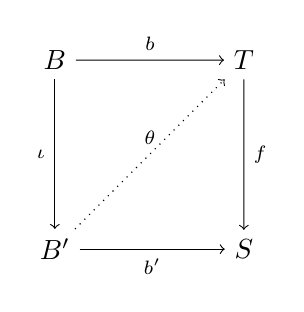
\begin{tikzpicture}[scale=0.8]
		
	\node (B') at (0,0) {$B'$};
	\node (B) at (0,3) {$B$};
	\node (S) at (3,0) {$S$};
	\node (T) at (3,3) {$T$};
	
	
	\path[->,font=\scriptsize]
		(B) edge node[left]{$\iota$} (B')
		(B') edge node[below]{$b'$} (S)
		(T) edge node[right]{$f$} (S)
		(B) edge node[above]{$b$} (T);
		
	\path[->, font = \scriptsize, dotted]
		(B') edge node[above]{$\theta$} (T);
			
\end{tikzpicture}


  			\end{center}
		\end{figure}
		 
		 When there is an open morphism $\map{f}{T}{S}$, then $T$ and $S$ are bisimilar. Indeed, the relation $R = \{(p,f(p)) \mid p$ is accessible$\}$, where we say that $p$ is accessible iff there is an execution $\map{b}{B}{T}$ of size $n$ with $b(n) = p$, is a bisimulation.
		 % we have already seen it is a simulation, so we must prove that if there is a transition $(f(p),a,q')$ in $S$ with $p$ accessible from $i$ then there is a transition $(p,a,p')$ in $T$ with $f(p') = q'$. Indeed, let $\map{b}{B}{T}$ be an execution, with $B = (\textbf{[n]},0,\Delta)$ and $b(n) = p$. Define $B' = (\textbf{[n+1]},0,\Delta')$ with $\Delta' = \Delta\cup\{(n,a,n+1)\}$ and $\map{b'}{B'}{S}$ which maps $i \leq n$ to $f(b(i))$ and $n+1$ to $q'$. This is a morphism since $f$, $b$ are morphisms, $f(b(n)) = f(p)$ and $(f(p),a,q')$ is a transition in $S$. So we have a diagram as required in the definition of an open map. So since $f$ is open there is such a $\map{\theta}{B'}{T}$. In particular, if we note $p' = \theta(n+1)$, then $f(p') = f\circ\theta(n+1) = b'(n+1) = q'$ and $(p,a,p') = (\theta(n),a,\theta(n+1))$ is a transition in $T$.
		 
		 This result can be strengthened as follow: two systems $T$ and $S$ are bisimilar iff there is a span of open maps between them, i.e., there are a system $U$ and open maps $\map{f}{U}{T}$ and $\map{g}{U}{S}$. We have already seen that open morphisms induce bisimulations so if there is a span of open maps between two systems, they are bisimilar. Reciprocally, if $R$ is a bisimulation between $T$ and $S$, define $U = (R,(i,i'),\Delta'')$ where $\Delta'' = \{((p,q),a,(p',q')) \mid (p,a,p') \in \Delta \wedge (q,a,q') \in \Delta'\}$, and $f$ (resp. $g$) being the first (resp. second) projection. It is easy to check that $f$ and $g$ are open.
		 
		 This view was developed in \cite{joyal96} and was applied in other models than transition systems. We will see other occurrences of this theory later on.
		 
		 
		 \subsection{Coalgebraic view}
		 
		 This starts with the following observation \cite{jacobs16}: a transition system is a set $Q$ of states together with two functions
		 \begin{itemize}
		 	\item $\map{i}{\ast}{Q}$, where $\ast$ is a singleton (initial state),
			\item $\map{\Delta}{Q}{\mathcal{P}(\Sigma\times Q)}$, where $\mathcal{P}(X)$ is the set of subsets of $X$ (transitions).
		\end{itemize}
		So a transition system consists of a bialgebra $\ast \rightarrow Q \rightarrow \mathcal{P}(\Sigma\times Q)$, more precisely, a set $Q$, an $F$-algebra on $Q$ with 
		$$\map{F}{\setcat}{\setcat} ~~~ X \mapsto \ast$$
		and a $G$-coalgebra on $Q$ with
		$$\map{G}{\setcat}{\setcat} ~~~ X \mapsto \mathcal{P}(\Sigma\times X)$$
		Given two endofunctors on the same category $\C$, $F,G$-bialgebras form a category whose morphisms from $F(X) \xrightarrow{~f_1~} X \xrightarrow{~f_2~} G(X)$ to $F(Y) \xrightarrow{~g_1~} Y \xrightarrow{~g_2~} G(Y)$ are morphisms $h$ of $\C$ from $X$ to $Y$ such that:
		
		\begin{figure}[H]
			\begin{center}
    				
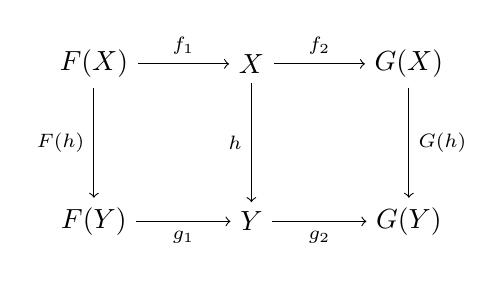
\begin{tikzpicture}[scale=1]
		
	\node (fx) at (0,0) {$F(X)$};
	\node (fy) at (0,-2) {$F(Y)$};
	\node (x) at (2,0) {$X$};
	\node (y) at (2,-2) {$Y$};
	\node (gx) at (4,0) {$G(X)$};
	\node (gy) at (4,-2) {$G(Y)$};
	
	\path[->,font=\scriptsize]
		(fx) edge node[left]{$F(h)$} (fy)
		(x) edge node[left]{$h$} (y)
		(gx) edge node[right]{$G(h)$} (gy)
		(fx) edge node[above]{$f_1$} (x)
		(x) edge node[above]{$f_2$} (gx)
		(fy) edge node[below]{$g_1$} (y)
		(y) edge node[below]{$g_2$} (gy);
			
\end{tikzpicture}


  			\end{center}
		\end{figure}
		
		In the case of transition systems seen as $F,G$-bialgebras, a morphism $f$ of $F,G$-bialgebra from $T$ to $S$ is a morphism of transition systems with the extra property that for every transition of the form $(f(p),a,q')$ in $S$, there is a transition $(p,a,p')$ in $T$ with $f(p') = q'$. In this case, morphisms of $F,G$-bialgebra do not coincide with open morphisms. They will when every state of $T$ is accessible. So a similar result holds: two transition systems are bisimilar iff there is a span of $F,G$-bialgebras morphisms between them. 
		
		\begin{figure}[H]
			\begin{center}
    				
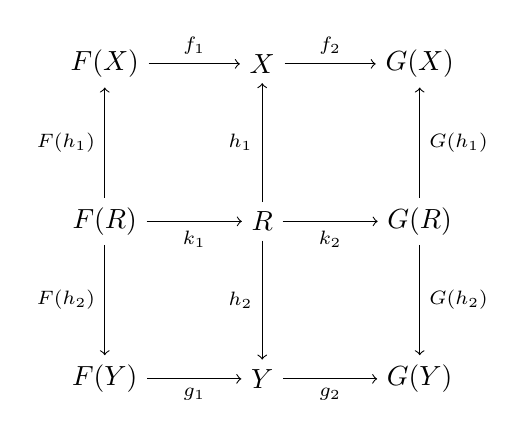
\begin{tikzpicture}[scale=1]
		
	\node (fx) at (0,0) {$F(X)$};
	\node (fr) at (0,-2) {$F(R)$};
	\node (fy) at (0,-4) {$F(Y)$};
	\node (x) at (2,0) {$X$};
	\node (r) at (2,-2) {$R$};
	\node (y) at (2,-4) {$Y$};
	\node (gx) at (4,0) {$G(X)$};
	\node (gr) at (4,-2) {$G(R)$};
	\node (gy) at (4,-4) {$G(Y)$};
	
	\path[->,font=\scriptsize]
		(fr) edge node[left]{$F(h_1)$} (fx)
		(r) edge node[left]{$h_1$} (x)
		(gr) edge node[right]{$G(h_1)$} (gx)
		(fr) edge node[left]{$F(h_2)$} (fy)
		(r) edge node[left]{$h_2$} (y)
		(gr) edge node[right]{$G(h_2)$} (gy)
		(fx) edge node[above]{$f_1$} (x)
		(x) edge node[above]{$f_2$} (gx)
		(fy) edge node[below]{$g_1$} (y)
		(y) edge node[below]{$g_2$} (gy)
		(fr) edge node[below]{$k_1$} (r)
		(r) edge node[below]{$k_2$} (gr);
			
\end{tikzpicture}


  			\end{center}
		\end{figure}
		
		 
		 




\section{Semantic for true concurrency}
\label{sec:semtc}

In this section, we see how bisimilarity can be defined in true concurrency: this will involve unfolding and event structures. We end the section with a discussion of the notion of actions and its refinements.

	\subsection{Unfolding of transition systems}
	
	The unfolding of a transition system is an equivalent system without loops, obtained by ``unfolding'' the loops. More precisely, it is a synchronisation tree which is bisimilar to the transition system. Given a transition system $T = (Q,i,\Delta)$, the unfolding $\mathrm{Unfold}(T)$ of $T$ is the transition system $(P, j, \Gamma)$ where:
\begin{itemize}
	\item $P = \{(q_0, a_1, q_1, \ldots, a_n, q_n)\mid q_i \in Q, \, a_i \in \Sigma, \, (q_i, a_{i+1}, q_{i+1}) \in \Delta \wedge q_0 = i\}$
	\item $j = (i)$
	\item $\Gamma = \{((q_0, a_1, q_1, \ldots, a_n, q_n),b,(q_0, a_1, q_1, \ldots, a_n, q_n,b,q))\mid (q_n,b,q) \in \Delta\}$
\end{itemize}
It is easy to check that $\{(q_n,(q_0, a_1, q_1, \ldots, a_n, q_n)) \mid (q_0, a_1, q_1, \ldots, a_n, q_n) \in P\wedge q_0 = i\}$ is a bisimulation between $T$ and $\mathrm{Unfold}(T)$.\\
Equivalently, the unfolding of $T$ can be defined as a glueing of all branches of $T$, i.e., in terms of colimits. We will look at a generalization to other categories of systems in Chapter 3. Unfolding is then the right adjoint of the inclusion of trees in these systems.

	\subsection{Event structures and unfolding of TSI}

	This will be similar in transition systems with independence: unfolding is the right adjoint of some inclusion. Event structures will play the role of trees in this case. A \textbf{($\Sigma$-labelled) event structure} is a tuple $S = (E,\leq,\text{Cons},\lambda)$ where:
	\begin{itemize}
		\item a set $E$ of \textbf{events},
		\item a partial order $\leq$ on $E$, called the \textbf{causal dependency order},
		\item a set $\text{Cons}$ of finite subsets of $E$, called the \textbf{consistency relation},
		\item a function $\map{\lambda}{E}{\Sigma}$, the \textbf{labelling}.
	\end{itemize}
\noindent which satisfies that:
	\begin{itemize}
		\item for every event $e$, the set $\{e' \mid e' \leq e\}$ is finite (finite cause),
		\item for every event $e$, $\{e\} \in \text{Cons}$,
		\item if $Y \subseteq X$ and $X \in \text{Cons}$, then $Y \in \text{Cons}$,
		\item if $X \in \text{Cons}$, for every pair of events $e \leq e'$ with $e' \in X$, $X\cup\{e\} \in \text{Cons}$.
	\end{itemize}
	
\noindent An event structure induces a transition system with independence  as follow:
	\begin{itemize}
		\item its states are the \textbf{configurations}, that is finite downward-closed sets $C$ of events in $\text{Cons}$,
		\item transitions are triples $(C,a,C')$ such that $C' = C \sqcup \{e\}$ with $\lambda(e) = a$,
		\item its initial state is the empty set,
		\item the independence relation is the set of pairs $((C,a,C'),(D,b,D'))$ such that if $C' = C \sqcup \{e\}$ and $D' = D \sqcup \{e'\}$, $e$ and $e'$ are \textbf{concurrent} meaning that $e \not\leq e'$, $e'\not\leq e$ and $\{e,e'\} \in \text{Cons}$.
	\end{itemize}
	This construction extends to a coreflexion from a category of event structures to a category of transition systems with independence \cite{nielsen94}. Its right adjoint is what is called the \textbf{unfolding}. Intuitively, it is constructed as a system whose states are executions modulo $\simeq$.
	
	\subsection{Bisimulations of event structures}
	
	Bisimulations of event structures thus induce bisimulations on transition systems with independence through this unfolding. A \textbf{history-preserving bisimulation} \cite{rabinovitch88} between two event structures $S$ and $T$ consists of a set $R$ of triples $(C,f,C')$ with $C$ a configuration of $S$, $C'$ a configuration of $T$ and $\map{f}{C}{C'}$ an isomorphism of posets, such that:
	\begin{itemize}
		\item $(\varnothing,\varnothing,\varnothing) \in R$,
		\item for every $(C,f,C') \in R$, for every event $e$ such that $C\sqcup\{e\}$ is a configuration with $\lambda(e) = a$, there is an event $e'$ such that $C'\sqcup\{e'\}$ is a configuration with $\lambda(e') = a$, and there is an isomorphism of posets $\map{f'}{C\cup\{e\}}{C'\cup\{e'\}}$ that extends $f$ and such that $(C\cup\{e\},f',C'\cup\{e'\}) \in R$,
		\item symmetrically.
	\end{itemize}
\noindent We say that $R$ is \textbf{strong} if furthermore:
	\begin{itemize}
		\item if $(C,f,C') \in R$, $D \subseteq C$ and if $\map{f'}{D}{D'}$ is the restriction of $f$ on $D$, then $(D,f',D') \in R$,
		\item symmetrically.
	\end{itemize}
\noindent We then say that two event structures are \textbf{(strong) hp bisimilar} if there is a (strong) history-preserving bisimulation between them. By extension, we say that two transition systems with independence are \textbf{(strong) hp bisimilar} if their unfoldings are. Equivalent definitions of hp bisimilarity and strong hp bisimilarity were investigated in \cite{joyal96}, in particular a logical view, a more classical definition using relations directly on the system, not on the unfolding, and a fibrational view.

	\subsection{Action refinement}
	\label{subsec:actref}

Until now, we have seen bisimulations as equivalence relations of systems with specified actions. But the notion of actions depends on the degree of abstractions. For example, summing two integers can be seen as an action on its own or as a sequence of smaller operations on digits. So a system can be modeled in different ways, depending on how fine-grained the actions are considered. An important property for systems and their bisimulations is that if two systems are bisimilar, then they must be bisimilar whatever is the granularity of actions. 

Let us look at an easy example. Let $T = (Q,i,\Delta)$ be a $\Sigma$-transition system and $a \in \Sigma$. Suppose that the action $a$ can be decomposed into a finite sequence of smaller actions $a_1$, \ldots, $a_n$. We can transform $T$ into another transition system $T'$ by replacing every transition $(q,a,q') \in \Delta$ by a sequence of transitions $(q,a_1,q_1)$, \ldots, $(q_i, a_{i+1},q_{i+1})$, \ldots, $(q_{n-1}, a_n, q')$, where $q_1$, \ldots, $q_{n-1}$ are fresh new states. It is then easy to prove that if two transition systems $T$ and $S$ are bisimilar, then $T'$ and $S'$ obtained by replacing $a$ by $a_1$, \ldots, $a_n$ are bisimilar.

This example is simple, because we only replace some actions by a linear sequence of actions, but we may imagine replacing actions by any transition system (with a final state).

This idea of replacing actions by more complicated objects have been formalized for event structures in \cite{vanglabbeek01}. A \textbf{refinement function} ref is a function from $\Sigma$ to particular event structures (namely \textbf{prime} event structures). One can then refine an event structure by modifying events in such a way that action $a$ of $\Sigma$ is decomposed into actions of $\text{ref}(a)$. One of the main result from \cite{vanglabbeek01} is that if two event structures are (strong) bisimilar then their refinements by any refinement function are (strong) hp bisimilar. We say that (strong) hp bisimilarity is invariant under action refinement.





\section{Higher Dimensional Automata (HDA)}
\label{sec:hda}

In Sections \ref{subsec:ats} and \ref{subsec:tsi}, we have seen extensions of transition systems in which we specify transitions or events that are independent. This independence allows us to specify that two actions are done simultaneously, and can be depicted by squares of the form:
	
				\begin{figure}[H]
					\begin{center}
    						
\begin{tikzpicture}[scale=1]
		
	\node (q) at (0,0) {$q$};
	\node (q') at (3,0) {$q'$};
	\node (p) at (0,3) {$p$};
	\node (p') at (3,3) {$p'$};
	
	\path[bend right = 45]
		(0.5,0.1) edge (0.1,0.5)
		(0.1,2.5) edge (0.5,2.9)
		(2.9,0.5) edge (2.5,0.1)
		(2.5,2.9) edge (2.9,2.5);
	
	\path[->,font=\scriptsize]
		(q) edge node[below]{$a$} (q')
		(p) edge node[above]{$a$} (p')
		(q) edge node[left]{$b$} (p)
		(q') edge node[right]{$b$} (p');
			
\end{tikzpicture}


  					\end{center}
				\end{figure}
				
	The idea of higher dimensional automata (HDA for short) \cite{pratt91}, is to specify those squares (and more generally, cubes of any dimension) explicitly. In this section, we present those HDA, their unfolding and bisimulations.

	\subsection{The formalism}

	A \textbf{precubical set} is a sequence $(Q_n)_{n\in \nat}$ of sets together with functions:
	$$\map{\partial_i^\alpha}{Q_n}{Q_{n-1}}$$
	for $n \in \nat$, $1 \leq i \leq n$ and $\alpha \in \{0,1\}$, satisfying for every $1 \leq i < j \leq n$ and $\alpha, \beta \in \{0,1\}$:
	$$\partial_i^\alpha\circ\partial_j^\beta = \partial_{j-1}^\beta\circ\partial_i^\alpha.$$
	A \textbf{higher dimensional automata} is a tuple $(Q,\partial, i, \lambda)$ with:
	\begin{itemize}
		\item $(Q,\partial)$  a precubical set,
		\item $i \in Q_0$ (\textbf{initial state}),
		\item $\map{\lambda}{Q_1}{\Sigma}$ (\textbf{labelling}), such that for every $c \in Q_2$ and $i \in \{1,2\}$:
			$$\lambda(\partial_i^0(c)) = \lambda(\partial_i^1(c)).$$
				
				\begin{figure}[H]
					\begin{center}
    						
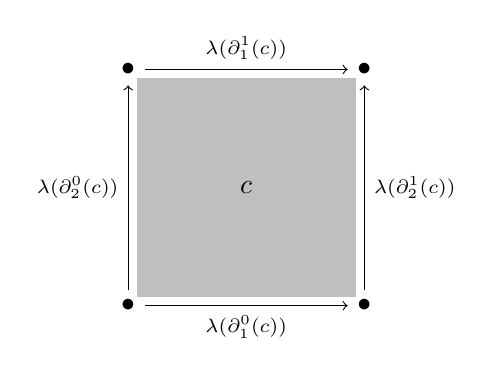
\begin{tikzpicture}[scale=1]
		
	\node (11) at (0,0) {$\bullet$};
	\node (12) at (0,3) {$\bullet$};
	\node (21) at (3,0) {$\bullet$};
	\node (22) at (3,3) {$\bullet$};
	
	\draw[draw = white, fill = gray!50] (0.1,0.1) rectangle (2.9,2.9);
	
	\node (c) at (1.5,1.5) {$c$};
	
	\path[->,font=\scriptsize]
		(11) edge node[left]{$\lambda(\partial_2^0(c))$} (12)
		(21) edge node[right]{$\lambda(\partial_2^1(c))$} (22)
		(11) edge node[below]{$\lambda(\partial_1^0(c))$} (21)
		(12) edge node[above]{$\lambda(\partial_1^1(c))$} (22);
			
\end{tikzpicture}


  					\end{center}
				\end{figure}
	\end{itemize}
	
	HDA are the most powerful models for concurrency. \cite{vanglabbeek05} translated many models for concurrency into HDA in a way that preserves behaviors. Those constructions were improved in \cite{goubault12} to make them adjunctions, extending the work from \cite{nielsen95}.

	
	\subsection{Paths, homotopy and unfolding}
	
	Paths are similar to branches seen previously, and represent executions of the system: they will be sequences of actions, some potentially simultaneous, except that an action is not required to terminate before another can start. For example, an action $a$ may be started, then an action $b$ is started, then the action $b$ is terminated, then the action $a$ is terminated. More precisely \cite{vanglabbeek05}, a \textbf{path} $\pi$ in an HDA $(Q,\partial,i,\lambda)$ is a sequence $(t_1,c_1), \ldots, (t_n,c_n)$, depicted as $$i = c_0 \xrightarrow{~t_1~} c_1 \xrightarrow{~t_2~} \ldots \xrightarrow{~t_n~} c_n$$
	where:
	\begin{itemize}
		\item $c_k \in Q$,
		\item $t_k$ is of the form $\partial_{j_k}^{\alpha_k}$,
		\item if $\alpha_k = 0$, then $t_k(c_{k-1}) = c_k$, with $t_k(c_k) = c_{k-1}$ otherwise.
	\end{itemize}

	
	For example, if we consider the following HDA:
	
				\begin{figure}[H]
					\begin{center}
    						
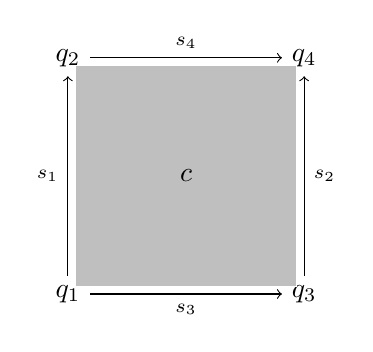
\begin{tikzpicture}[scale=1]
		
	\node (11) at (0,0) {$q_1$};
	\node (12) at (0,3) {$q_2$};
	\node (21) at (3,0) {$q_3$};
	\node (22) at (3,3) {$q_4$};
	
	\draw[draw = white, fill = gray!50] (0.1,0.1) rectangle (2.9,2.9);
	
	\node (c) at (1.5,1.5) {$c$};
	
	\path[->,font=\scriptsize]
		(11) edge node[left]{$s_1$} (12)
		(21) edge node[right]{$s_2$} (22)
		(11) edge node[below]{$s_3$} (21)
		(12) edge node[above]{$s_4$} (22);
			
\end{tikzpicture}


  					\end{center}
				\end{figure}
				
\noindent with $i = q_1$, $\lambda(s_1) = \lambda(s_2) = a$ and $\lambda(s_3) = \lambda(s_4) = b$, and if we want to formalize the previous execution, that is, starting $a$, starting $b$, ending $b$, ending $a$, we will consider the path:
	$$(\partial_1^0,s_1), (\partial_2^0, c), (\partial_2^1,s_2), (\partial_1^1,q_4)$$
	which geometrically can be depicted as follow (in red):
	
				\begin{figure}[H]
					\begin{center}
    						
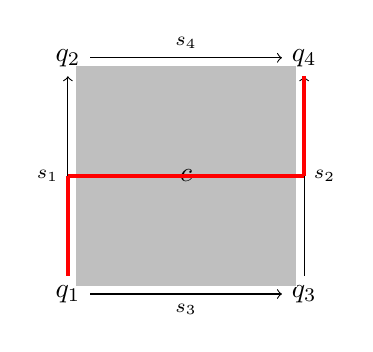
\begin{tikzpicture}[scale=1]
		
	\node (11) at (0,0) {$q_1$};
	\node (12) at (0,3) {$q_2$};
	\node (21) at (3,0) {$q_3$};
	\node (22) at (3,3) {$q_4$};
	
	\draw[draw = white, fill = gray!50] (0.1,0.1) rectangle (2.9,2.9);
	
	\node (c) at (1.5,1.5) {$c$};
	
	\path[->,font=\scriptsize]
		(11) edge node[left]{$s_1$} (12)
		(21) edge node[right]{$s_2$} (22)
		(11) edge node[below]{$s_3$} (21)
		(12) edge node[above]{$s_4$} (22);
		
	\path[very thick, red]
		(11) edge (0,1.5)
		(0,1.5) edge (3,1.5)
		(3,1.5) edge (22);
			
\end{tikzpicture}


  					\end{center}
				\end{figure}

				
	Homotopy is a way to express that two paths represent the same execution modulo permutations of independent actions. It is similar to the relation $\simeq$ defined for executions of transition systems with independence. It will be defined by saying that two paths are equivalent if one can deform one into the other by doing elementary modifications, which consist essentially in permuting two independent elements of a path. A path $\pi = i \xrightarrow{~t_1~} c_1 \xrightarrow{~t_2~} \ldots \xrightarrow{~t_n~} c_n$ is elementary homotopic to $\pi' = i \xrightarrow{~t'_1~} c'_1 \xrightarrow{~t'_2~} \ldots \xrightarrow{~t'_n~} c'_n$ if there are $1 \leq j \leq n-1$ and $k < l$ such that for every $p \neq j$ $c_p = c'_p$, for every $r \notin \{j, j+1\}$ $t_r = t'_r$ and one of the following occurs:
		\begin{itemize}
			\item $t_j = \partial_k^0$, $t_{j+1} = \partial_l^0$, $t'_j = \partial_{l-1}^0$ and $t'_{j+1} = \partial_k^0$,
			\item $t_j = \partial_k^1$, $t_{j+1} = \partial_l^1$, $t'_j = \partial_{l-1}^1$ and $t'_{j+1} = \partial_k^1$,
			\item $t_j = \partial_k^0$, $t_{j+1} = \partial_l^1$, $t'_j = \partial_{l-1}^1$ and $t'_{j+1} = \partial_k^0$,
			\item $t_j = \partial_l^0$, $t_{j+1} = \partial_k^1$, $t'_j = \partial_{k}^1$ and $t'_{j+1} = \partial_{l-1}^0$.
		\end{itemize}
	We call \textbf{homotopy} the reflexive, symmetric, transitive closure of elementary homotopy. In this case, we say that the paths are \textbf{homotopic} \cite{vanglabbeek05}.

	
	Geometrically, in the 2-dimensional case, elementary homotopy can be depicted as follow:
	
				\begin{figure}[H]
					\begin{center}
    						
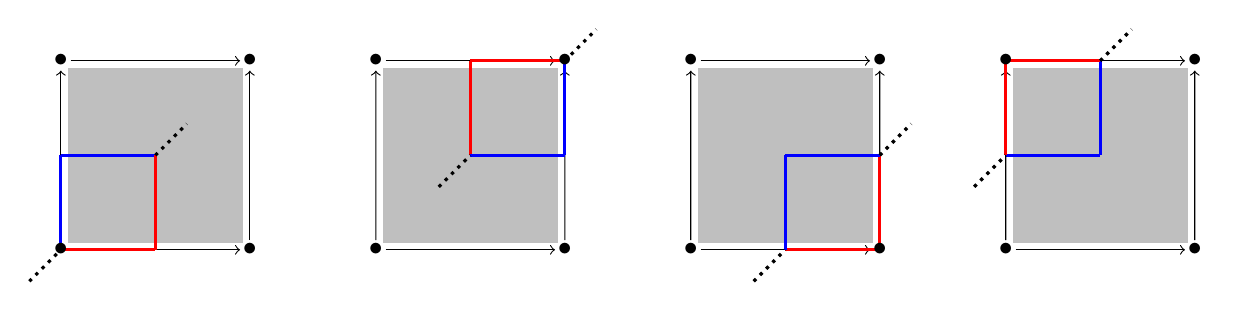
\begin{tikzpicture}[scale=0.8]

	\node (11) at (0,0) {};
	\node (12) at (0,3) {};
	\node (21) at (3,0) {};
	\node (22) at (3,3) {};
	
	\draw[draw = white, fill = gray!50] (0.1,0.1) rectangle (2.9,2.9);
	
	\path[->,font=\scriptsize]
		(11) edge (12)
		(21) edge (22)
		(11) edge (21)
		(12) edge (22);
		
	\path[very thick, blue]
		(0,0) edge (0,1.5)
		(0,1.5) edge (1.5,1.5);
		
	\path[very thick, red]
		(0,0) edge (1.5,0)
		(1.5,0) edge (1.5,1.5);
		
	\path[very thick, dotted]
		(-0.5,-0.5) edge (0,0)
		(1.5,1.5) edge (2,2);
		
	\node at (0,0) {$\bullet$};
	\node at (0,3) {$\bullet$};
	\node at (3,0) {$\bullet$};
	\node at (3,3) {$\bullet$};
	
	
	
	
	\node (11p) at (5,0) {};
	\node (12p) at (5,3) {};
	\node (21p) at (8,0) {};
	\node (22p) at (8,3) {};
	
	\draw[draw = white, fill = gray!50] (5.1,0.1) rectangle (7.9,2.9);
	
	\path[->,font=\scriptsize]
		(11p) edge (12p)
		(21p) edge (22p)
		(11p) edge (21p)
		(12p) edge (22p);
		
	\path[very thick, red]
		(6.5,1.5) edge (6.5,3)
		(6.5,3) edge (8,3);
		
	\path[very thick, blue]
		(6.5,1.5) edge (8,1.5)
		(8,1.5) edge (8,3);
		
	\path[very thick, dotted]
		(6,1) edge (6.5,1.5)
		(8,3) edge (8.5,3.5);
		
	\node at (5,0) {$\bullet$};
	\node at (5,3) {$\bullet$};
	\node at (8,0) {$\bullet$};
	\node at (8,3) {$\bullet$};
	
	
	
	
	\node (11pp) at (10,0) {};
	\node (12pp) at (10,3) {};
	\node (21pp) at (13,0) {};
	\node (22pp) at (13,3) {};
	
	\draw[draw = white, fill = gray!50] (10.1,0.1) rectangle (12.9,2.9);
	
	\path[->,font=\scriptsize]
		(11pp) edge (12pp)
		(21pp) edge (22pp)
		(11pp) edge (21pp)
		(12pp) edge (22pp);
		
	\path[very thick, red]
		(11.5,0) edge (13,0)
		(13,0) edge (13,1.5);
		
	\path[very thick, blue]
		(11.5,0) edge (11.5,1.5)
		(11.5,1.5) edge (13,1.5);
		
	\path[very thick, dotted]
		(11,-0.5) edge (11.5,0)
		(13,1.5) edge (13.5,2);
		
	\node at (10,0) {$\bullet$};
	\node at (10,3) {$\bullet$};
	\node at (13,0) {$\bullet$};
	\node at (13,3) {$\bullet$};
	
	
	
	
	\node (11ppp) at (15,0) {};
	\node (12ppp) at (15,3) {};
	\node (21ppp) at (18,0) {};
	\node (22ppp) at (18,3) {};
	
	\draw[draw = white, fill = gray!50] (15.1,0.1) rectangle (17.9,2.9);
	
	\path[->,font=\scriptsize]
		(11ppp) edge (12ppp)
		(21ppp) edge (22ppp)
		(11ppp) edge (21ppp)
		(12ppp) edge (22ppp);
		
	\path[very thick, blue]
		(15,1.5) edge (16.5,1.5)
		(16.5,1.5) edge (16.5,3);
		
	\path[very thick, red]
		(15,1.5) edge (15,3)
		(15,3) edge (16.5,3);
		
	\path[very thick, dotted]
		(14.5,1) edge (15,1.5)
		(16.5,3) edge (17,3.5);
		
	\node at (15,0) {$\bullet$};
	\node at (15,3) {$\bullet$};
	\node at (18,0) {$\bullet$};
	\node at (18,3) {$\bullet$};
			
\end{tikzpicture}


  					\end{center}
				\end{figure}
	
\noindent where the four conditions consist in replacing the blue part by the red part.
	
	Unfolding is also similar to the one from transition systems. It is defined as an HDA of paths modulo homotopy \cite{vanglabbeek91}. The \textbf{unfolding} of an HDA $(Q,\partial, i, \lambda)$ is the HDA $(Q', \partial', i', \lambda')$ where:
	\begin{itemize}
		\item $Q'_n$ is the set of homotopy class of paths $i \xrightarrow{~t_1~} c_1 \xrightarrow{~t_2~} \ldots \xrightarrow{~t_k~} c_k$ with $c_k \in Q_n$,
		\item $i'$ is the homotopy class of the constant path (which corresponds to the empty sequence),
		\item $\lambda([i \xrightarrow{~t_1~} c_1 \xrightarrow{~t_2~} \ldots \xrightarrow{~t_k~} c_k]) = \lambda(c_k)$,
		\item $\partial_i^1([i \xrightarrow{~t_1~} c_1 \xrightarrow{~t_2~} \ldots \xrightarrow{~t_k~} c_k]) = [i \xrightarrow{~t_1~} c_1 \xrightarrow{~t_2~} \ldots \xrightarrow{~t_k~} c_k \xrightarrow{~\partial_i^1~} \partial_i^1(c_k)]$,
		\item $\partial^0_i([i \xrightarrow{~t_1~} c_1 \xrightarrow{~t_2~} \ldots \xrightarrow{~t_k~} c_k]) = [\pi]$ where $\pi$ is a path such that $\pi \xrightarrow{~\partial_i^0~} c_k$ is homotopic to $i \xrightarrow{~t_1~} c_1 \xrightarrow{~t_2~} \ldots \xrightarrow{~t_k~} c_k$.
	\end{itemize}

	
	
	\subsection{Bisimilarities}
	
	There are several definitions of bisimilarity of HDA \cite{vanglabbeek05}, which use the same pool of axioms. They are based on a particular observation of a path. First, the \textbf{split-trace} of a path, is the sequence of labellings of actions started and terminated along the path. For example, the split-trace of the path from the previous example would be $a_+.b_+.b_-.a_-$, meaning that an $a$ action is started, then a $b$ action is started, then a $b$ action is terminated and finally an $a$ action is terminated. But this observation is partial since if several $a$ actions are started, when an $a$ action is terminated, denoted by $a_-$, we do not know which one is terminated. The \textbf{ST-trace} is an improvement of the split-trace in which the $a_-$ are replaced by $a_k$ where $k$ denotes which action is terminated. For example, a path of the form ``a first $a$ action is started ; a second $a$ action is started ; the second $a$ action is terminated ; the first $a$ action is terminated'' would have a ST-trace of the form $a_+.a_+.a_2.a_1$. A \textbf{bisimulation} between two HDA is a relation $R$ between paths which satisfies some of those axioms:
	\begin{enumerate}
		\item the empty paths are related,
		\item if two paths are related then their ST-traces are the same,
		\item if $(\pi,\pi') \in R$ and $\rho$ is homotopic to $\pi$, then there is $\rho'$ homotopic to $\pi'$ such that $(\rho,\rho')\in R$,
		\item symmetrically,
		\item if $(\pi,\pi') \in R$ and $\pi$ is a prefix of $\rho$, then $\pi'$ is a prefix of some $\rho'$ such that $(\rho,\rho') \in R$,
		\item symmetrically,
		\item if $(\pi,\pi') \in R$ and $\rho$ is a prefix of $\pi$, then there is a prefix $\rho'$ of $\pi'$ such that $(\rho,\rho')$,
		\item symmetrically.
	\end{enumerate}
\noindent When $R$ satisfies:
	\begin{itemize}
		\item $1-8$, we say that the HDA are \textbf{hereditary history-preserving bisimilar} (hhp-bisimilar for short),
		\item $1-6$, we say that the HDA are \textbf{history-preserving bisimilar} (hp-bisimilar for short),
		\item $1-2$ and $5-8$, we say that the HDA are \textbf{ST-bisimilar}. In this case, $7-8$ are consequences of the other axioms.
	\end{itemize}
Easily, hhp implies hp which implies ST and the other implications do not hold.

There is another notion of bisimulation from \cite{fahrenberg14} which is based on the fibrational view from Section \ref{subsubsec:fibra}.
	



\section{SU and PV-programs}
\label{sec:supv}

In the following, we describe two languages which concretely talk about true concurrency: the SU-programs \cite{afek90} and the PV-programs \cite{dijkstra65}. For both, we also describe how they can be translated in HDA or TSI.


	\subsection{SU-programs}

Assume that we have $n$ processes, $A_1$, ..., $A_n$ running in parallel and that those processes have access to a global memory. Each possesses its own part of the memory and those parts form a partition of the global memory.

				\begin{figure}[H]
					\begin{center}
    						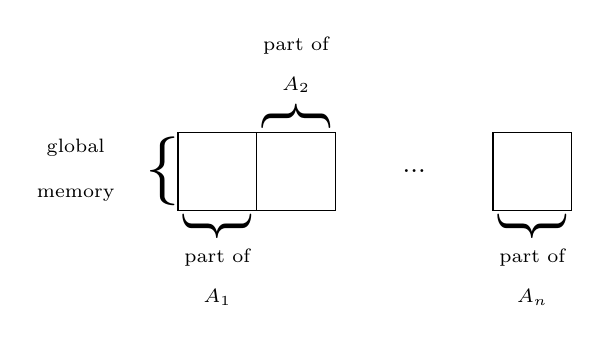
\begin{tikzpicture}[scale=1]
		
					\draw (0,0) rectangle (1,1);
					\draw (1,0) rectangle (2,1);
					\draw (4,0) rectangle (5,1);
					\node at (-1.3,0.8) {\scriptsize{global}};
					\node at (-1.3,0.2) {\scriptsize{memory}};
					\node at (-0.2,0.5) {\Huge{\{}};
					\node at (0.5,-0.2) {\rotatebox{90}{\Huge{\{}}};
					\node at (1.5,1.2) {\rotatebox{90}{\Huge{\}}}};
					\node at (4.5,-0.2) {\rotatebox{90}{\Huge{\{}}};
					\node at (3,0.5) {...};
					\node at (0.5,-0.6) {\scriptsize{part of}};
					\node at (0.5,-1.1) {\scriptsize{$A_1$}};
					\node at (1.5,2.1) {\scriptsize{part of}};
					\node at (1.5,1.6) {\scriptsize{$A_2$}};
					\node at (4.5,-0.6) {\scriptsize{part of}};
					\node at (4.5,-1.1) {\scriptsize{$A_n$}};
			
\end{tikzpicture}
  					\end{center}
				\end{figure}

Each process can do two types of actions on the memory:
\begin{itemize}
	\item \textbf{S-actions}, which consist in \textbf{scanning} the whole global memory,
	\item \textbf{U-actions}, which consist in \textbf{updating} their own part of the memory.
\end{itemize}

The processes can also globally synchronize, in the sense that they all wait until every process has finished its execution until a certain point of the program. So a SU-program with $n$ processes $P$ will be a term generated by the following grammar:

$$P ::= Q_1\parallel \ldots \parallel Q_n \mid P\bullet P$$
$$Q_1, \ldots, Q_n, Q ::= S.Q \mid U.Q \mid \varepsilon$$

For example, $(S.S\parallel U.S)\bullet(U\parallel S.U)$ stands for a SU-program with 2 processes. The first one does 2 S-actions while the second does a U-action then an S-action. At this point, they synchronize, that is, they wait until the other has finished this part of the program. Then, the first does a U-action while the other does an S-action followed by a U-action. 

There is a translation from SU-programs to transition systems with independence (and so to HDA). Start with a program of the form $Q_1\parallel \ldots \parallel Q_m$. Let $k_i$ be the size of $Q_i$, that is, the number of $S$ and $U$ in it and denote $Q_i[j]$ the $j$-th letter of $Q_i$. The states of this program are $\{0, \ldots, k_1\}\times\ldots\{0,\ldots, k_m\}$. There is exactly one transition from $(j_1, \ldots, j_i, \ldots, j_m)$ to $(j_1, \ldots, j_i +1, \ldots, j_m)$ and it is labelled by $Q_i[j_i+1]$. Two transitions are independent if and only if either they are both labelled by S, or both by U. The intuition is the following: if two processes are doing an action simultaneously, thre are three possible cases:
\begin{itemize}
	\item they are both S-actions: in this case, since the memory is not changed, there is no problem,
	\item they are both U-actions: in this case, since disjoint parts of the memory are changed, there is no problem,
	\item one is an S-action and the other is a U-action: in this case, one process is scanning the memory while the other is changing its part, which makes the value of the memory scanned unpredictable. There is a problem.
\end{itemize}
Now, if we have a program of the form $P_1\bullet P_2 \bullet \ldots \bullet P_m$, with $P_i$ containing no $\bullet$, the transition system associated with this program is obtained by considering the transition systems for every $P_i$ as defined above and then identifying the state $(k_1, \ldots, k_m)$ of $P_i$ with the state $(0, \ldots, 0)$ of $P_{i+1}$.

For example, using the geometric picture from HDA, the SU-program $(S.S\parallel U.S)\bullet(U\parallel S.U)$ can be seen as:

				\begin{figure}[H]
					\begin{center}
    						
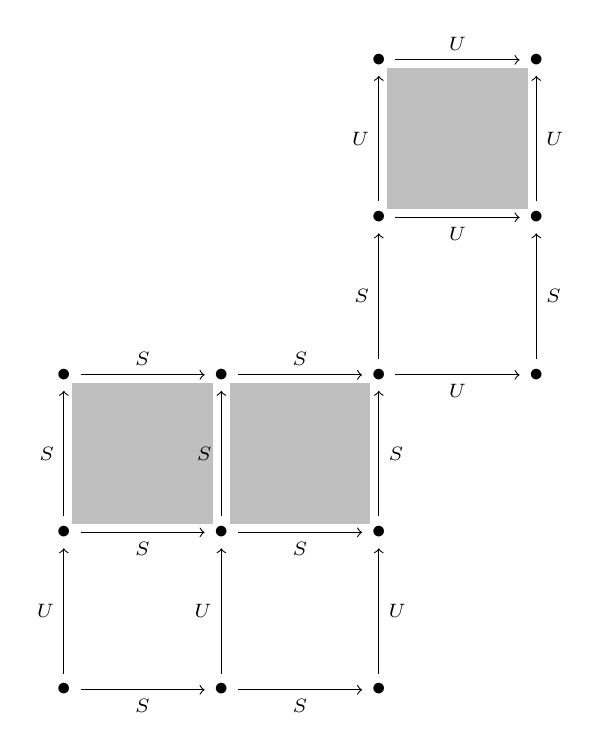
\begin{tikzpicture}[scale=1]
		
	\node (00) at (0,0) {$\bullet$};
	\node (01) at (2,0) {$\bullet$};
	\node (02) at (4,0) {$\bullet$};
	\node (10) at (0,2) {$\bullet$};
	\node (11) at (2,2) {$\bullet$};
	\node (12) at (4,2) {$\bullet$};
	\node (20) at (0,4) {$\bullet$};
	\node (21) at (2,4) {$\bullet$};
	\node (22) at (4,4) {$\bullet$};
	\node (23) at (6,4) {$\bullet$};
	\node (32) at (4,6) {$\bullet$};
	\node (33) at (6,6) {$\bullet$};
	\node (42) at (4,8) {$\bullet$};
	\node (43) at (6,8) {$\bullet$};
	
	\draw[draw = white, fill = gray!50] (0.1,2.1) rectangle (1.9,3.9);
	\draw[draw = white, fill = gray!50] (2.1,2.1) rectangle (3.9,3.9);
	\draw[draw = white, fill = gray!50] (4.1,6.1) rectangle (5.9,7.9);

	\path[->,font=\scriptsize]
		(00) edge node[below]{$S$} (01)
		(01) edge node[below]{$S$} (02)
		(10) edge node[below]{$S$} (11)
		(11) edge node[below]{$S$} (12)
		(20) edge node[above]{$S$} (21)
		(21) edge node[above]{$S$} (22)
		(00) edge node[left]{$U$} (10)
		(10) edge node[left]{$S$} (20)
		(01) edge node[left]{$U$} (11)
		(11) edge node[left]{$S$} (21)
		(02) edge node[right]{$U$} (12)
		(12) edge node[right]{$S$} (22)
		(22) edge node[below]{$U$} (23)
		(32) edge node[below]{$U$} (33)
		(42) edge node[above]{$U$} (43)
		(22) edge node[left]{$S$} (32)
		(23) edge node[right]{$S$} (33)
		(32) edge node[left]{$U$} (42)
		(33) edge node[right]{$U$} (43);
			
\end{tikzpicture}


  					\end{center}
				\end{figure}
				 

	\subsection{PV-programs}
	
In this language, we assume that we have $n$ processes $A_1$, ..., $A_n$ running in parallel and that, this time, those processes can concurrently access $m$ resources $R_1$, ..., $R_m$. Each resource has a capacity $\nu_i$, which is an integer in $\{1,\ldots, n-1\}$ which represents the maximal number of processes that can have access to this resource simultaneously.

A process can do two types of actions:
\begin{itemize}
	\item \textbf{$P_i$-actions}, which consist in asking for access to the resource $R_i$,
	\vspace{-0.4cm} \item[or] ~
	\vspace{-0.4cm} \item \textbf{$V_i$-actions}, which consist in freeing access to the resource $R_i$.
\end{itemize}

Between those actions, the processes can do local actions that are independent of each other and are seen as silent actions. The processes can also globally synchronize, in the same sense as SU-programs. So a PV-program with $n$ processes $P$ will be a term generated by the following grammar:

$$P ::= Q_1\parallel \ldots \parallel Q_n \mid P\bullet P$$
$$Q_1, \ldots, Q_n, Q ::= P_i.Q \mid V_i.Q \mid \varepsilon$$

Much as SU-programs, PV-programs can be translated into transition systems with independence. For an explicit construction, see \cite{fajstrup16}. Let us illustrate this on an example.

Consider the program $P_1.P_2.V_2.V_1\parallel P_2.P_1.V_1.V_2$ with $\nu_1 = \nu_2 = 1$. The two processes cannot have simultaneous access to the resources. This program is modeled by the following transition system with independence. Start by constructing the following grid:
				\begin{figure}[H]
					\begin{center}
    						
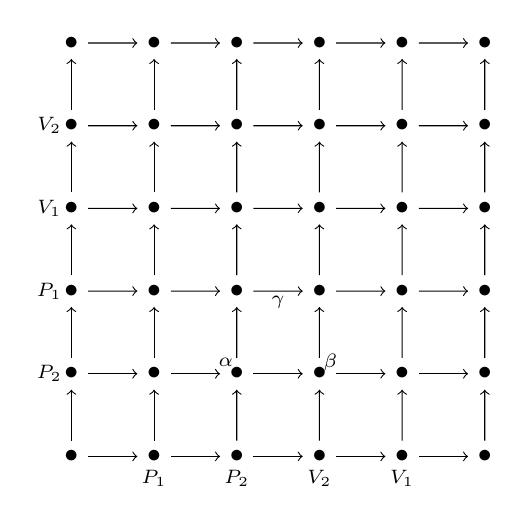
\begin{tikzpicture}[scale=0.7]
		
	\foreach \x in {0,...,5}
   		 \foreach \y in {0,...,5} 
      			 \node  (\x\y) at (1.5*\x,1.5*\y) {$\bullet$};
	\foreach \x in {0,...,5}
   		 \foreach \y [count=\yi] in {0,...,4}  
     			 {\draw[->] (\x\y)--(\x\yi) ;
			 \draw[->] (\y\x)--(\yi\x) ;}
	
	\node (al) at (2.8,1.7) {\scriptsize{$\alpha$}};
	\node (be) at (4.7,1.7) {\scriptsize{$\beta$}};
	\node (ga) at (3.75,2.8) {\scriptsize{$\gamma$}};
	\node (p11) at (1.5,-0.4) {\scriptsize{$P_1$}};
	\node (p21) at (3,-0.4) {\scriptsize{$P_2$}};
	\node (v21) at (4.5,-0.4) {\scriptsize{$V_2$}};
	\node (v11) at (6,-0.4) {\scriptsize{$V_1$}};
	\node (p22) at (-0.4,1.5) {\scriptsize{$P_2$}};
	\node (p12) at (-0.4,3) {\scriptsize{$P_1$}};
	\node (v12) at (-0.4,4.5) {\scriptsize{$V_1$}};
	\node (v22) at (-0.4,6) {\scriptsize{$V_2$}};
	
	
			
\end{tikzpicture}


  					\end{center}
				\end{figure}
For example, the state $\alpha$ corresponds to a state where horizontal process has the access to the first resource, and both processes ask for the access to the second resource but do not get it yet; the state $\beta$ corresponds to a state where the horizontal process has access to the first resource, had the access to the second resource but has released it, and the vertical process still waiting for the access to the second resource; and so on. Every state corresponds to a valid configuration of the program, meaning that there is no state where both processes have access to the same resource. However, there are transitions that are not possible. For example, the transition $\gamma$ corresponds to a sequence of configurations where the horizontal process starts by waiting for the access to the second resource, gains it and finishes by releasing it, while the vertical process has the access to the second resource. So the only possible transitions are:
				\begin{figure}[H]
					\begin{center}
    						
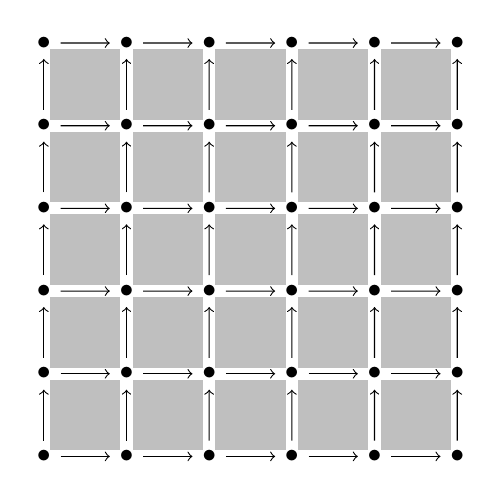
\begin{tikzpicture}[scale=0.7]
		
	\foreach \x in {0,...,5}
   		 \foreach \y in {0,...,5} 
      			 \node  (\x\y) at (1.5*\x,1.5*\y) {$\bullet$};
	\foreach \x in {0,...,5}
   		 \foreach \y [count=\yi] in {0,...,4}  
     			 {\ifthenelse{2 = \x \AND  2 = \y}{}
			 	{\ifthenelse{3 = \x \AND 2 = \y}{}{\draw[->] (\x\y)-- (\x\yi); \draw[->] (\y\x)-- (\yi\x);}}}
				
	\foreach \x [count=\xi] in {0,...,4}
   		 \foreach \y [count=\yi] in {0,...,4}  
		 	{\ifthenelse{2 = \x \AND 2 = \y}{}
				{\ifthenelse{1 = \x \AND 2 = \y}{}
					{\ifthenelse{2 = \x \AND 1 = \y}{}
						{\ifthenelse{2 = \x \AND 3 = \y}{}
							{\ifthenelse{3 = \x \AND 2 = \y}{}
			{\draw[draw = white, fill = gray!50] {(\x\y)+(0.1,0.1)} rectangle (1.5*\xi-0.1,1.5*\yi-0.1);}}}}}}
     			 
				
	
	
			
\end{tikzpicture}


  					\end{center}
				\end{figure}
\noindent and since we assume that the operations other than P and V are all independent, all squares are independent meaning that in the HDA we have 2-dimensional squares as depicted above.




